%%%%%%%%%%%%%%%%%%%%%%%%%%%%%%%%%%%%%%%%%%%%%%%%%%%%%%%%%%%%%%%%%%%%%
% LaTeX Template: Project Titlepage Modified (v 0.1) by rcx
%
% Original Source: http://www.howtotex.com
% Date: February 2014
% 
% This is a title page template which be used for articles & reports.
% 
% This is the modified version of the original Latex template from
% aforementioned website.
% 
%%%%%%%%%%%%%%%%%%%%%%%%%%%%%%%%%%%%%%%%%%%%%%%%%%%%%%%%%%%%%%%%%%%%%%

\documentclass[12pt]{report}
\usepackage[a4paper]{geometry}
\usepackage[myheadings]{fullpage}
\usepackage{fancyhdr}
\usepackage{lastpage}
\usepackage{graphicx, wrapfig, subcaption, setspace, booktabs}
\usepackage[T1]{fontenc}
\usepackage[font=small, labelfont=bf]{caption}
\usepackage{fourier}
\usepackage[protrusion=true, expansion=true]{microtype}
\usepackage[english]{babel}
\usepackage{sectsty}
\usepackage{url, lipsum}
\usepackage{graphicx}

\newcommand{\HRule}[1]{\rule{\linewidth}{#1}}
\onehalfspacing
\setcounter{tocdepth}{5}
\setcounter{secnumdepth}{5}

%-------------------------------------------------------------------------------
% HEADER & FOOTER
%-------------------------------------------------------------------------------
\pagestyle{fancy}
\fancyhf{}
\setlength\headheight{15pt}
\fancyhead[L]{Wang \& Ocampo }
\fancyhead[R]{Allegheny College }
\fancyfoot[R]{Page \thepage\ of \pageref{LastPage}}
%-------------------------------------------------------------------------------
% TITLE PAGE
%-------------------------------------------------------------------------------

\begin{document}


\title{Stock Market Analysis}

\author{
		Daniel Ocampo \\ 
		Henry Wang \\
		Department of Computer Sciences }
\date {
9th December, 2016
}
\maketitle
\tableofcontents
\newpage

%-------------------------------------------------------------------------------
% Section title formatting
\sectionfont{\scshape}
%-------------------------------------------------------------------------------

%-------------------------------------------------------------------------------
% BODY
%-------------------------------------------------------------------------------

\section{Introduction}


Our team decide to apply database to a real life problem on stock market. When we were trying to decide the topic for the final project, the first idea came to our mind was to collect data from the stock market and then analyze it to see if any negative impact has happened since the election. Once the project starts, we found that the data for one month was not enough for our project since we were dealing with stock market. So finally we collected 3 stock markets' data for the past 2 years.    
\section{Data Collection}
After collecting and comparing a few websites, we made our final decision on yahoo finance as our primary data source. The website contains the stock price from 1950 to 2016 by days. Also this website provides a visualization of data that we can have a guideline what's going on in the stock market visually. So we downloaded the data as csv file for 3 major market: NASDAQ Composite, Dow Jones Industrial Average, and S\&P 500.  When we were doing data collection, we also added primary key for each csv file so we were ready to build our tables and schemas for our database. Once we finished those data collection, and talked with Professor Bonham-Carter, we decided to add the data of unemployment rate into our research, so we found the data of unemployment rate U.S. Bureau of Labor Statistics, and created table and schemas for this data.


\section{Tables and schemas}
When we started to build our database, we built everything in SQLite (data.sqlite3) since this is the database software we use most frequently. We created tables in our setup.txt file based on the data we had, which contains date, open, high, low, closed, volume,adj, id for every stock table. The date is to store time information for the stock market. The open is to store the price on the open day of the stock market. The high is to store highest price the stock reached that day and then there's low. The closed is to store the price of the last trade when the market closes that day. The volume is to store the number of share traded that day. The adj means adjusted close which is to store the after hours price and the true open price adjusted from the close price posted. The id is the primary key for every table. For the unemployment rate table, we created the table base on the month and year, and we added id as a primary key. 
\section{ Software}

We used MAMP as our main database software. MAMP is a software that hosts websites with MySQL and apache. MAMP allows the user to create tables, and import data through a user interfaces called phpMyAdmin. The first thing we had to solve is that we could not install the software on Linux which makes it very difficult to work as team. We downloaded MAMP on Windows 7 where most of the coding was done. The first part that we did was to figure out how to connect to the database using MAMP. Once connection is made, we were able to import the data, and had PHP query through the data using variables. The data would then be stored in an array where it then be printed out. Using PHP integrated with HTML allowed us to make drop down menus and user inputs. We were able to choose what data we wanted use. For example, if the user pressed one button, we have to specify what button is pressed and update the values of the button that has been pressed. We would get errors because we have defined variables that are not be used. That is okay because unlike java, our program We used MAMP as our main database software. MAMP is a software that hosts websites with MySQL and apache. MAMP allows the user to create tables, and import data through a user interfaces called phpMyAdmin. The first thing we had to solve is that we could not install the software on Linux which makes it very difficult to work as team. We downloaded MAMP on Windows 7 where most of the coding was done. The first part that we did was to figure out how to connect to the database using MAMP. Once connection is made, we were able to import the data, and had PHP query through the data using variables. The data would then be stored in an array where it then be printed out. Using PHP integrated with HTML allowed us to make drop down menus and user inputs. We were able to choose whatwill still run with errors.\\
\includegraphics[scale=.13]{table.png}
\\These are tables we had in MAMP.\\
\section{The Queries}
We created queries that would compare three major stock markets, to see if there is anything we could find. The first query just puts all of the stock market in order based on the starting date to the end data using the primary key. This part is probably the hardest one because our primary key was created as string that contains both an integer and string. We had to do cast it as an integer, and used some command as seen below. The second one is less complicated but we saw that this basic query for the the unemployment would best used if we were just to see it in order because it can cover large amounts of data in order. The third query that can be manipulated into two is suppose to tell us what were the the ultimate high and the ultimate lows for two stock markets. For example, if we chose the NASDAQ15 and NASDAQ16 then we would see which one is higher. We tried to figure out if there is a connection of when the stock market is high during those years. So if we see that for the past five years in the month of April the stocks were really high, for the two consecutive we would know to expect that next year will also be high or at the very least know that it is a high chance that it will be high. This query also works in the opposite direction where the user can choose whether they want to check the highs or the lows to see this pattern. The fouWe created queries that would compare three major stock markets, to see if there is anything we could find. The first query just puts all of the stock market in order based on the starting date to the end data using the primary key. This part is probably the hardest one because our primary key was created as string that contains both an integer and string. We had to do cast it as an integer, and used some command as seen below. The second one is less complicated but we saw that this basic query for the the unemployment would best used if we were just to see it in order because it can cover large amounts of data in order. The third query that can be manipulated into two is suppose to tell us what were the the ultimate high and the ultimate lows for two stock markets. For example, if we chose the NASDAQ15 and NASDAQ16 then we would see which one is higher. We tried to figure out if there is a connection of when the stock market is high during those years. So if we see that for the past five years in the month of April the stocks were really high, for the two consecutive we would know to expect that next year will also be high or at the very least know that it is a high chance that it will be high. This query also works in the opWe created queries that would compare three major stock markets, to see if there is anything we could find. The first query just puts all of the stock market in order based on the starting date to the end data using the primary key. This part is probably the hardest one because our primary key was created as string that contains both an integer and string. We had to do cast it as an integer, and used some command as seen below. The second one is less complicated but we saw that this basic query for the the unemployment would best used if we were just to see it in order because it can cover large amounts of data in order. The third query that can be manipulated into two is suppose to tell us what were the the ultimate high and the ultimate lows for two stock markets. For example, if we chose the NASDAQ15 and NASDAQ16 then we would see which one is higher. We tried to figure out if there is a connection of when the stock market is high during those years. So if we see that for the past five years in the month of April the stocks were really high, for the two consecutive we would know to expect that next year will also be high or at the very least know that it is a high chance that it will be high. This query also works in the opposite direction where the user can choose whether they want to check the highs or the lows to see this pattern. The fouposite direction where the user can choose whether they want to check the highs or the lows to see this pattern. The fourth query has three functions because it can check for equality, greater than, or less than. So we if would like to see how much growth has happened between the same stock we just call the stock and make it print out when the stock equaled that value. Or let's say you only want to invest when the stocks are at certain amount so to predict when it will be that amount you can use the equality checker. It will return you with the date of when it was that price. The you could see if it is consistent by checking it again with the year before.\\


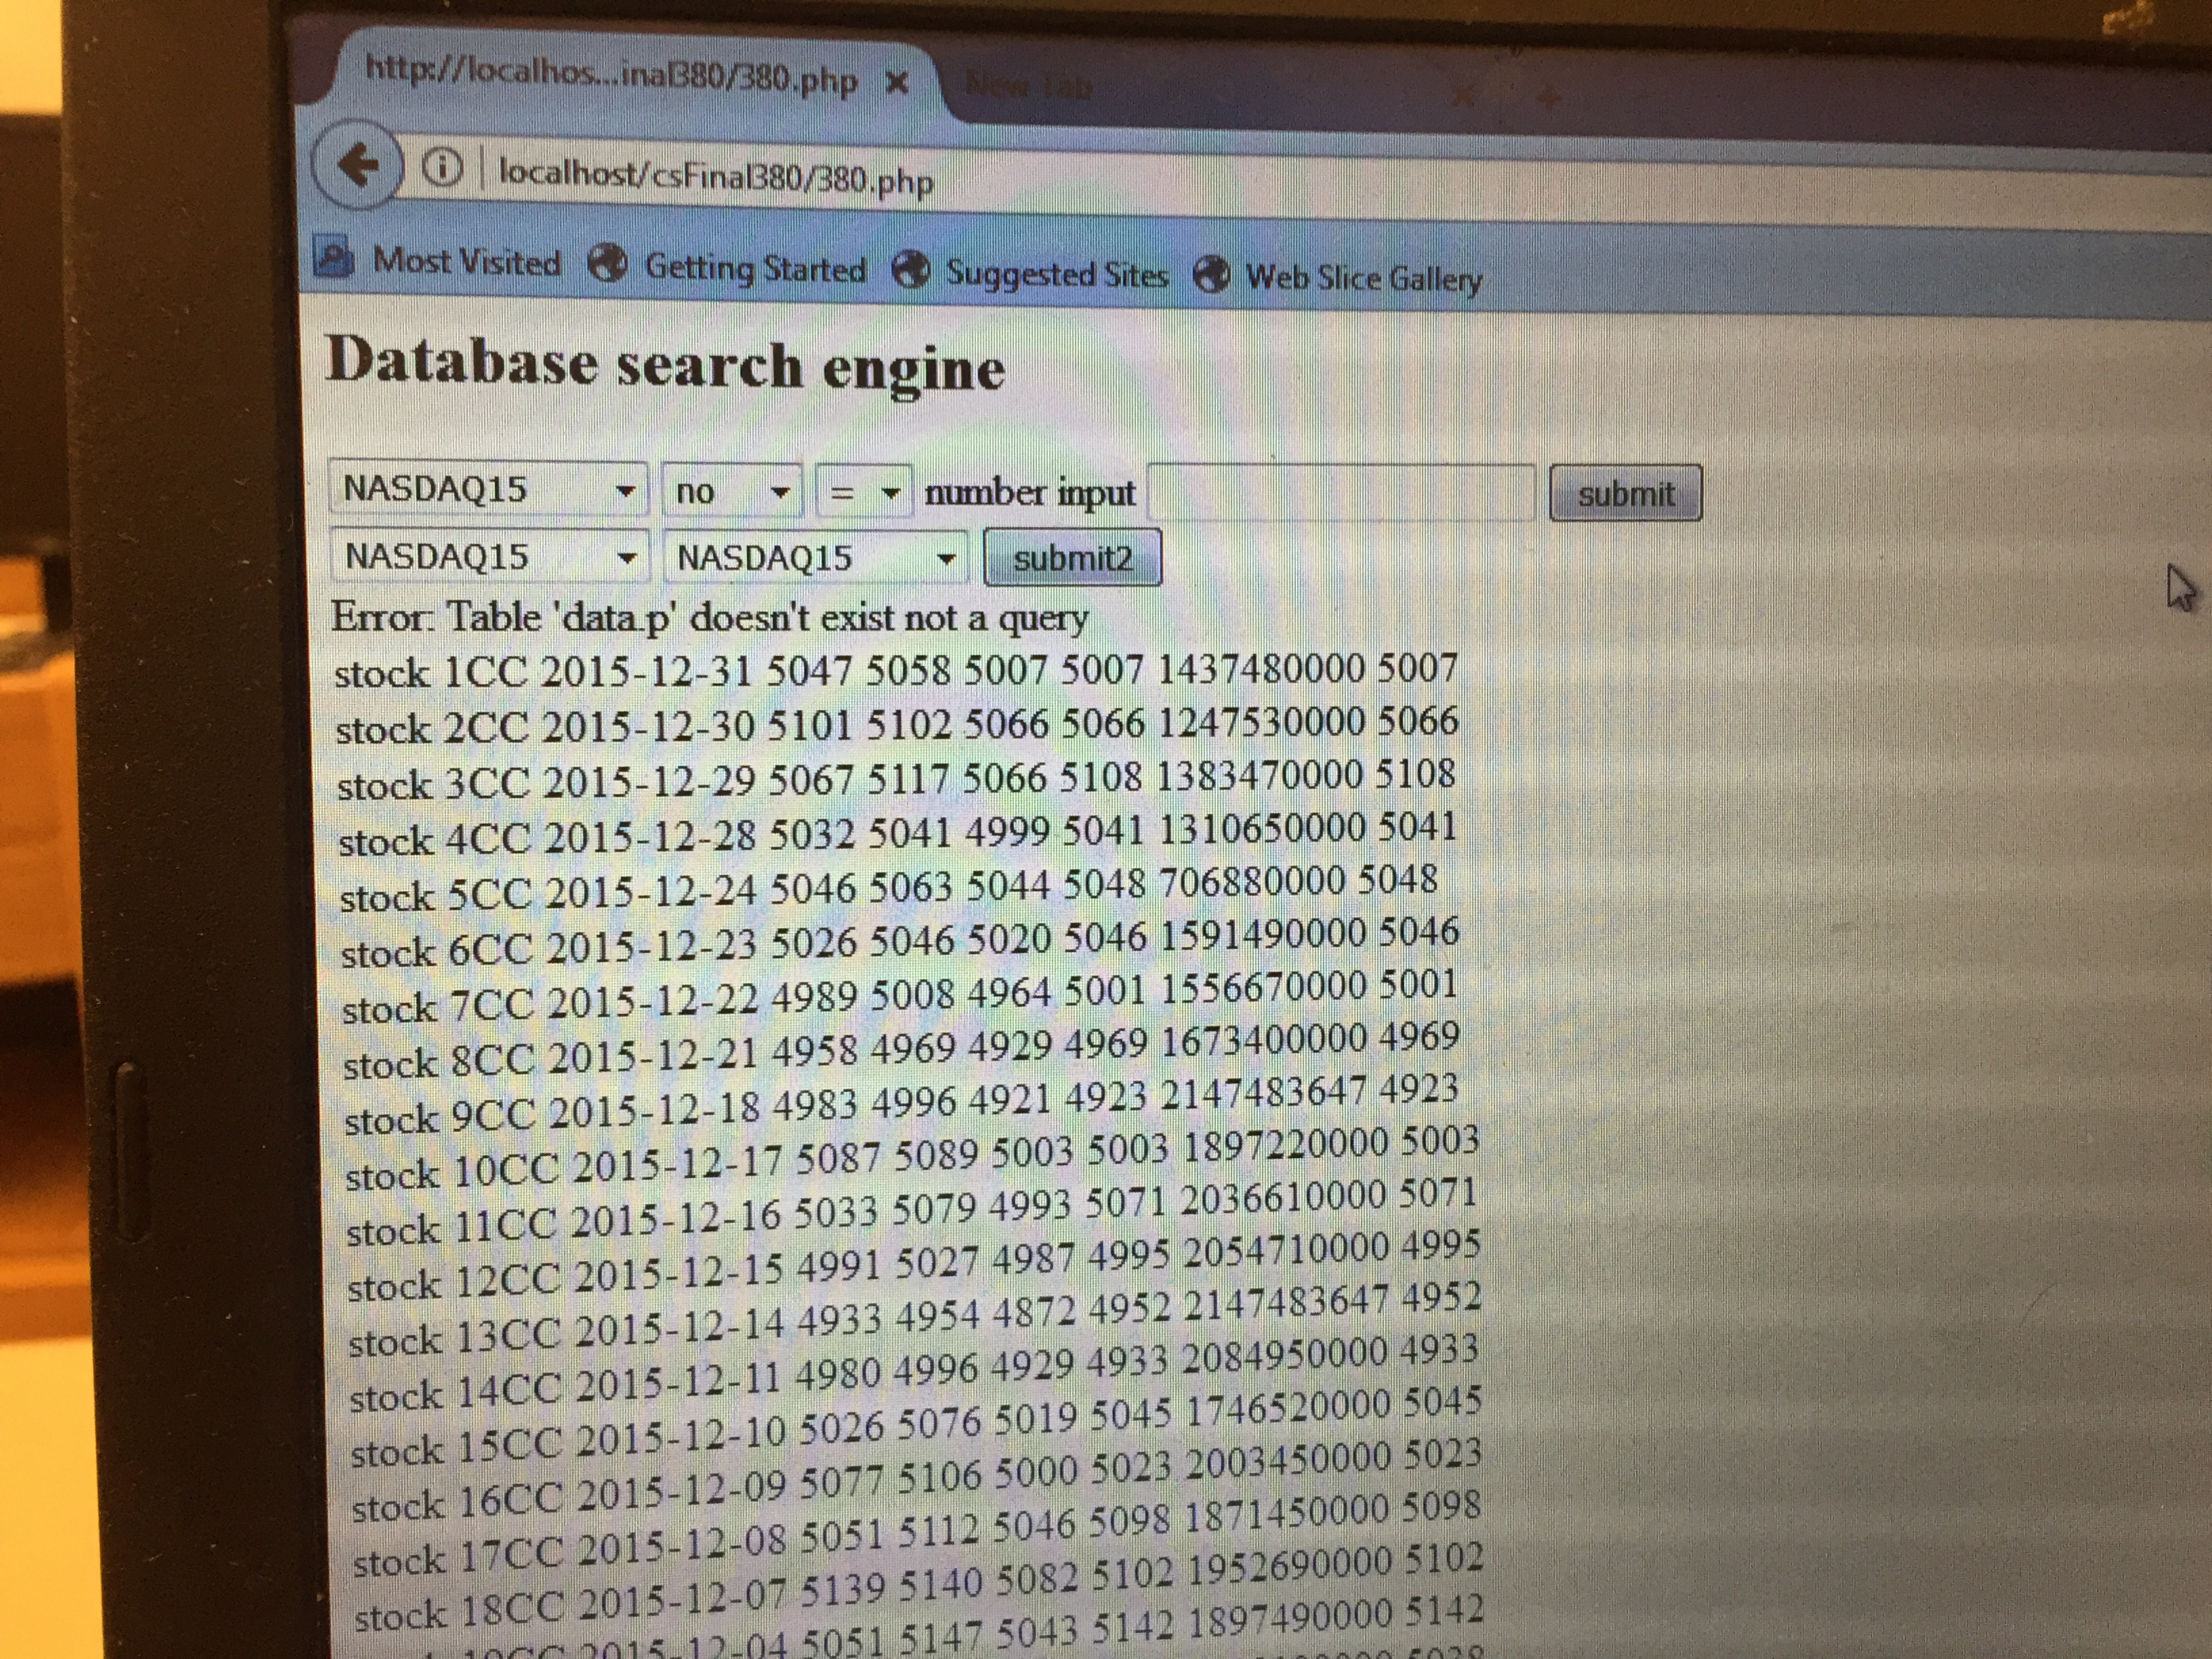
\includegraphics[scale=.13]{data.png}
\\This is the user inference in a php web page.\\
\begin{itemize}
\item select * from \$table order by CAST (ID signed INTEGER ) ASC;
\item select * from \$table order by ID ASC;
\item select n.date, p.date, n.high, from \$table1 p, \$table2 n where n.Date = p.Date order by p,high, n.high asc limit 10)
\item 4.select \$term , date, ID from \$table where \$term \$constraint \$number
\end{itemize}

\section{Our Discovery}

Based on the data we collected, we found there's more about the economy rather than buying stocks. Due to the fact that stock are complex to use, we had to do some research. We discovered that when stocks are up it meant the economy was doing very well. The unemployment rate was very low, and therefore the people's confidence was up. We noted that from the data we collected the unemployment rate was very high from 2008. We concluded the stocks must have been very low. Even though we did not collect that data from the stock market we are 100\% sure that it will be low. We also noticed that if a person invests the stocks they would likely get a average interest rate of 10\%, which is much higher than the bank's average interest rate. In the end we found that investing in the stock in good idea but a person should make an educated guess to to get the maximum profit. We also concluded that stock market is a complex system by querying the top 10 highest price in each stock market. We didn't use any data mining here because we have to know a lot of math and statistic to do it. However, we our tool is powerful enough that people working in banking can use it for future work.       

\section{Challenges and Final Thought}

First of all, we want to use this final project as an opportunity to learn new things and softwares about database. At the same time, we plan to solve a real life problem using database system. The first challenge we faced was how would we use the data from stock market. Once the project goes on, we found that the stock market is very complex, so we decided to find the relationship between the market itself and the unemployment rate. The second challenge was to learn PHP. The database software we were using, MAMP, is not too hard to use, but try to load, query,and build interface in PHP were a lot of work for both of us. We tried to do some data visualization in the webpage but it didn't work out because we couldn't figure out a best way to create graphs in PHP since we have a lot of data. If we can redo this project, we maybe choose python as our main software because I found an article in which the author used python to analyze the data from stock market. We do learning a lot from this project as a term, and we both think this is most useful final project in computer science that we ever did.
%-------------------------------------------------------------------------------
% REFERENCES
%-------------------------------------------------------------------------------
\newpage
\section*{References}
\addcontentsline{toc}{section}{References}

 
\begin{itemize}
\item "Yahoo Finance - Business Finance, Stock Market, Quotes, News." Yahoo! Yahoo!, n.d. Web. 8 Dec. 2016.

\item "Bureau of Labor Statistics Data." U.S. Bureau of Labor Statistics. U.S. Bureau of Labor Statistics, n.d. Web. 8 Dec. 2016 
\item @@NTGuardian. "An Introduction to Stock Market Data Analysis with Python (Part 1)." Curtis Miller's Personal Website. N.p., 26 Apr. 2016. Web. 8 Dec. 2016.

\end{itemize} 
 
\end{document}

%-------------------------------------------------------------------------------
% SNIPPETS
%-------------------------------------------------------------------------------

%\begin{figure}[!ht]
%	\centering
%	\includegraphics[width=0.8\textwidth]{file_name}
%	\caption{}
%	\centering
%	\label{label:file_name}
%\end{figure}

%\begin{figure}[!ht]
%	\centering
%	\includegraphics[width=0.8\textwidth]{graph}
%	\caption{Blood pressure ranges and associated level of hypertension (American Heart Association, 2013).}
%	\centering
%	\label{label:graph}
%\end{figure}

%\begin{wrapfigure}{r}{0.30\textwidth}
%	\vspace{-40pt}
%	\begin{center}
%		\includegraphics[width=0.29\textwidth]{file_name}
%	\end{center}
%	\vspace{-20pt}
%	\caption{}
%	\label{label:file_name}
%\end{wrapfigure}

%\begin{wrapfigure}{r}{0.45\textwidth}
%	\begin{center}
%		\includegraphics[width=0.29\textwidth]{manometer}
%	\end{center}
%	\caption{Aneroid sphygmomanometer with stethoscope (Medicalexpo, 2012).}
%	\label{label:manometer}
%\end{wrapfigure}

%\begin{table}[!ht]\footnotesize
%	\centering
%	\begin{tabular}{cccccc}
%	\toprule
%	\multicolumn{2}{c} {Pearson's correlation test} & \multicolumn{4}{c} {Independent t-test} \\
%	\midrule	
%	\multicolumn{2}{c} {Gender} & \multicolumn{2}{c} {Activity level} & \multicolumn{2}{c} {Gender} \\
%	\midrule
%	Males & Females & 1st level & 6th level & Males & Females \\
%	\midrule
%	\multicolumn{2}{c} {BMI vs. SP} & \multicolumn{2}{c} {Systolic pressure} & \multicolumn{2}{c} {Systolic Pressure} \\
%	\multicolumn{2}{c} {BMI vs. DP} & \multicolumn{2}{c} {Diastolic pressure} & \multicolumn{2}{c} {Diastolic pressure} \\
%	\multicolumn{2}{c} {BMI vs. MAP} & \multicolumn{2}{c} {MAP} & \multicolumn{2}{c} {MAP} \\
%	\multicolumn{2}{c} {W:H ratio vs. SP} & \multicolumn{2}{c} {BMI} & \multicolumn{2}{c} {BMI} \\
%	\multicolumn{2}{c} {W:H ratio vs. DP} & \multicolumn{2}{c} {W:H ratio} & \multicolumn{2}{c} {W:H ratio} \\
%	\multicolumn{2}{c} {W:H ratio vs. MAP} & \multicolumn{2}{c} {\% Body fat} & \multicolumn{2}{c} {\% Body fat} \\
%	\multicolumn{2}{c} {} & \multicolumn{2}{c} {Height} & \multicolumn{2}{c} {Height} \\
%	\multicolumn{2}{c} {} & \multicolumn{2}{c} {Weight} & \multicolumn{2}{c} {Weight} \\
%	\multicolumn{2}{c} {} & \multicolumn{2}{c} {Heart rate} & \multicolumn{2}{c} {Heart rate} \\
%	\bottomrule
%	\end{tabular}
%	\caption{Parameters that were analysed and related statistical test performed for current study. BMI - body mass index; SP - systolic pressure; DP - diastolic pressure; MAP - mean arterial pressure; W:H ratio - waist to hip ratio.}
%	\label{label:tests}
%\end{table}